%  \documentclass[DIV=12, a4]{scrartcl}
%\documentclass[12pt, a5]{scrartcl}
\documentclass[a4]{scrartcl}

\usepackage[
%fancytheorems, 
noindent, 
%spacingfix, 
%noheader
]{adam}

\usepackage{subfig}

\title{Numbers and Sets}
\subtitle{Adam Kelly}
\author{Lectured by Imre Leader}
\date{Michaelmas 2020}

\begin{document}

\maketitle

\begin{abstract}
	This document is an account of the Cambridge Mathematical Tripos course `Numbers and Sets', lectured by Prof. Imre Leader in Michaelmas 2020.
	This is a work in progress, and is likely to to contain errors, which you may assume to be my own.
	% This document is a rather brief summary of the first three chapters of H. S. M. Coxeter and S. L. Greitzer's `Geometry Revisited'.
	% In no ways is this fleshed out, and in most cases just contains the important results and diagrams.
	% Specifically, it's purpose is to be somewhat of a reference which one can consult whilst attempting olympiad geometry problems.
\end{abstract}

% {\small
% \textbf{Basic calculus} 

% Informal treatment of differentiation as a limit, the chain rule, Leibnitz's rule, Taylor series, informal treatment of \(O\) and \(o\) notation and l'Hôpital's rule; integration as an area, fundamental theorem of calculus, integration by substitution and parts. 

% Informal treatment of partial derivatives, geometrical interpretation, statement (only) of symmetry of mixed partial derivatives, chain rule, implicit differentiation. Informal treatment of differentials, including exact differentials. Differentiation of an integral with respect to a parameter.

% \textbf{First-order linear differential equations} 

% Equations with constant coefficients: exponential growth, comparison with discrete equations, series solution; modelling examples including radioactive decay.

% Equations with non-constant coefficients: solution by integrating factor.

% \textbf{Nonlinear first-order equations}

% Separable equations. Exact equations. Sketching solution trajectories. Equilibrium solutions, stability by perturbation; examples, including logistic equation and chemical kinetics. Discrete equations: equilibrium solutions, stability; examples including the logistic map.

% \textbf{Higher-order linear differential equations}

% Complementary function and particular integral, linear independence, Wronskian (for second-order equations), Abel's theorem. Equations with constant coefficients and examples including radioactive sequences, comparison in simple cases with difference equations, reduction of order, resonance, transients, damping. Homogeneous equations. Response to step and impulse function inputs; introduction to the notions of the Heaviside step-function and the Dirac delta-function. Series solutions including statement only of the need for the logarithmic solution.

% \textbf{Multivariate functions: applications}

% Directional derivatives and the gradient vector. Statement of Taylor series for functions on \(\mathbb{R}^{n} .\) Local extrema of real functions, classification using the Hessian matrix. Coupled first order systems: equivalence to single higher order equations; solution by matrix methods. Non-degenerate phase portraits local to equilibrium points; stability.

% Simple examples of first- and second-order partial differential equations, solution of the wave equation in the form \(f(x+c t)+g(x-c t)\).
% }

\tableofcontents

\clearpage
\section{Introduction}

Numbers and sets is one of the first course in pure mathematics that you will take
as an undergraduate at Cambridge. In a sense, it is the `starting course', in that it will introduce you to the `pure maths' way of thinking about things. 
This introduction will happen through the lense of thinking about objects, beginning with the natural and real numbers. You will be introduced to the `thoughtful way' of thinking about such objects, that you can carry through to almost every other course in pure mathematics.

\subsection{Structure of the Course}

This course is divided into four chapters.

\begin{enumerate}
	\item \emph{Elementary Number Theory}
	
	This is a chapter that almost everybody enjoys. 
	We deal with number theory first, which is elementary not in the sense that it is easy but in the sense that it is our `first steps' in the subject. The main aim of this chapter is to get used to the additive and multiplicative structure of the natural numbers.

	It is like that some of you will be familiar with this material already, but nothing in this chapter will be assumed, and everything will be built from the ground up.

	\item \emph{The Reals}
	
	This chapter has a different perspective, centering on the questions of \emph{what is a real number} and \emph{what can we assume about them?} This is one of the harder parts of this course, and many of the definitions contain a subtlety that is not present in other chapters. 

	\item \emph{Sets and Functions}
	
	This is a `terminology' chapter. There is no exciting theorems, mostly notation, definitions, and so on. It is a short chapter, but it is somewhat boring in that sense.

	\item \emph{Countability}
	
	This chapter is best described as `fun with infinite sets'. It is to do with the concepts introduced in Chapter 3 (in the sense that we are thinking about sets and functions), but it has a very different flavour. You will find results in this chapter that are both interesting and surprising. Almost everyone likes this chapter.
\end{enumerate}

Everything in the chapters above makes up the `course'. If you are wondering what is examinable, it will be everything in these lecture notes (unless otherwise stated). For a more formal answer to that question, have a look at \href{https://www.maths.cam.ac.uk/undergrad/files/schedules.pdf}{the schedules}.

\subsection{Books}

As with most mathematics courses in Cambridge, you will not need a textbook to follow this course. What is covered in lectures is enough to do both the example sheets and the examinations for this course. Still, you might find that a textbook can provide a different perspective, additional worked examples, and additional material that you may find informative, helpful or fun.

In particular, the following books are quite relevant/good, but there is no expectation that you will look at these.

\begin{itemize}
	\item R. T. Allenby, \emph{Numbers and Proofs}.
	
	This book is readable, easy to understand and clear.

	\item A. G. Hamilton, \emph{Numbers, Sets and Axioms}.
	
	Another readable and clear book, but with a different flavour to the previous book.

	\item H. Davenport, \emph{The Higher Arithmetic}.

	This book can be thought of as showing `where things go next'. It is very interesting, and goes quite a bit beyond this course. It is worth noting however that this book contains no exercises.
\end{itemize}

You should be able to find all of these books in either your college library or the university library.

\subsection{Example Sheets}

As is normal for a 24 lecture course, there will be 4 example sheets. You should be able to have a good go at the first one after lecture 3 or 4.






% \clearpage
% \section{Introduction}

% In many ways, differential equations is a course that studies the mathematics of change.
% Differential equations are central to many branches of mathematics and science (physics, biology, etc).

% \subsection{The History of Differential Equations}

% There is a long history of studying differential equations at Cambridge.
% Two notable 

% \clearpage
% \section{Points and Lines Connected with a Triangle}

% \begin{theorem}[Extended Law of Sines]
% 	For a triangle $ABC$ with circumradius $R$,
% 	$$
% 	\frac{a}{\sin A} = \frac{b}{\sin B} = \frac{c}{\sin C} = 2R
% 	$$
% \end{theorem}

% \begin{theorem}[Ceva's Theorem]
% 	Three cevians $AX$, $BY$, $CZ$, one through each vertex of a triangle $ABC$, are concurrent if and only if
% 	$$
% 	\frac{BX}{XC} \cdot \frac{CY}{YA}\cdot \frac{ZA}{ZB} = 1.
% 	$$
% \end{theorem}
% \begin{center}
% 	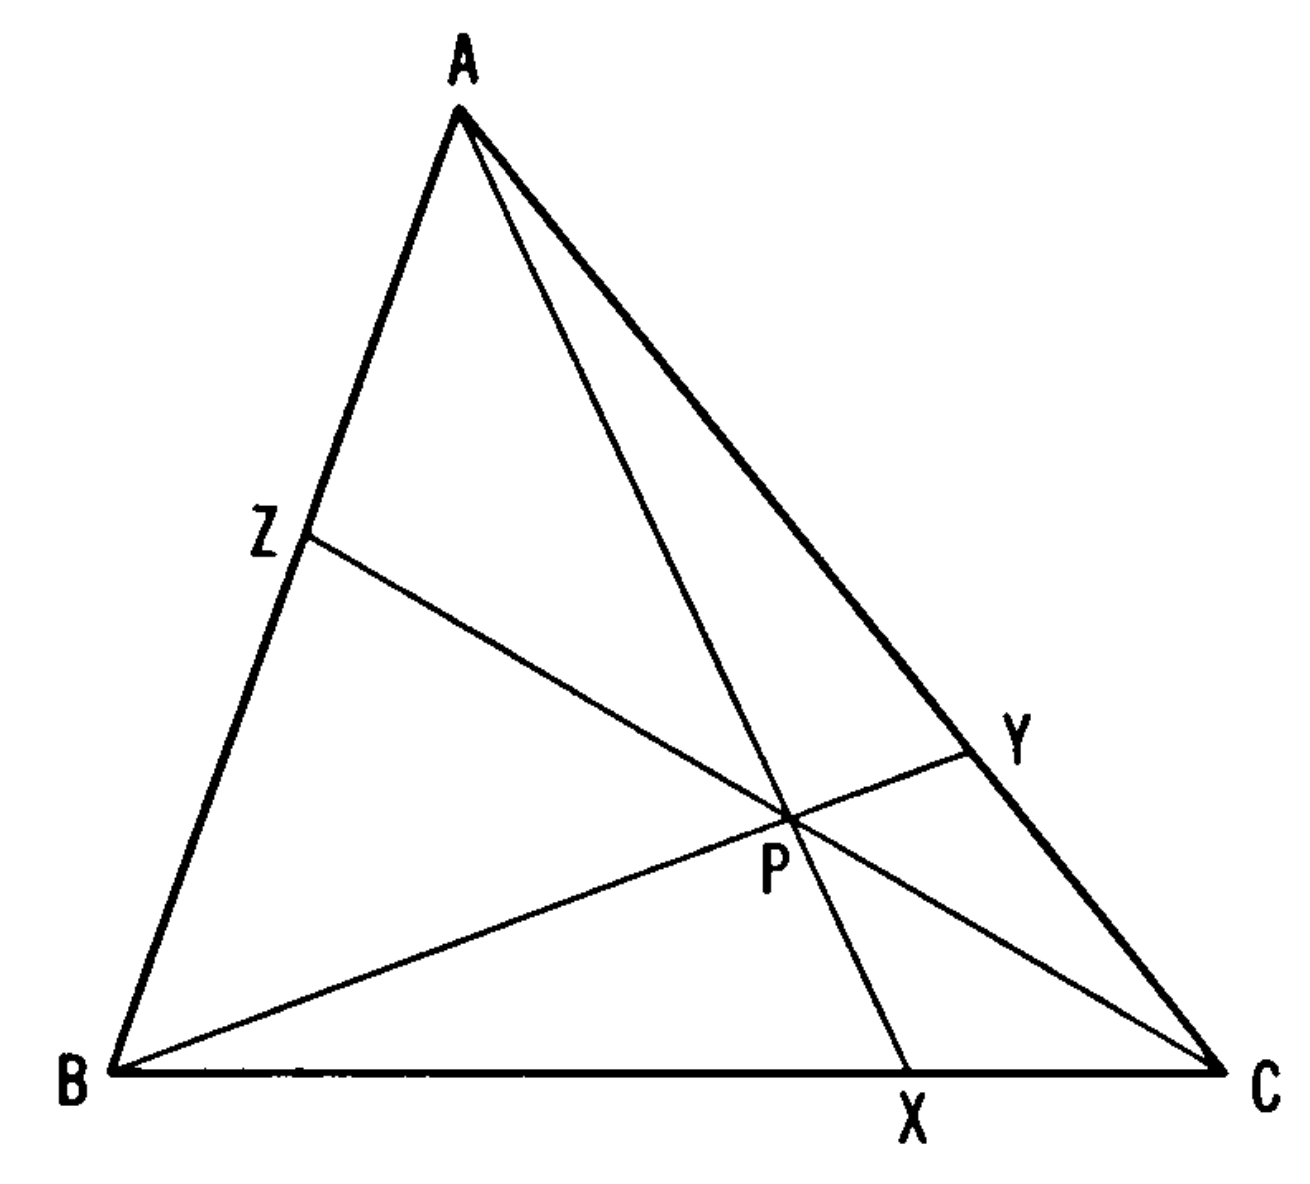
\includegraphics[width=0.35\textwidth]{media/1-2A}
% \end{center}

% \subsection{Points of Interest}

% \subsubsection{The Circumcenter}

% \begin{definition}
% 	The centre of the circle circumscribed about a triangle is the \vocab{circumcenter} of the triangle, and the circle is the \vocab{circumcircle}. 
% \end{definition}
% The circumcenter $O$ is the intersection of the three perpendicular bisectors of the sides of the triangles. Typically the radius of the circumcircle is denoted $R$.
% \begin{center}
% 		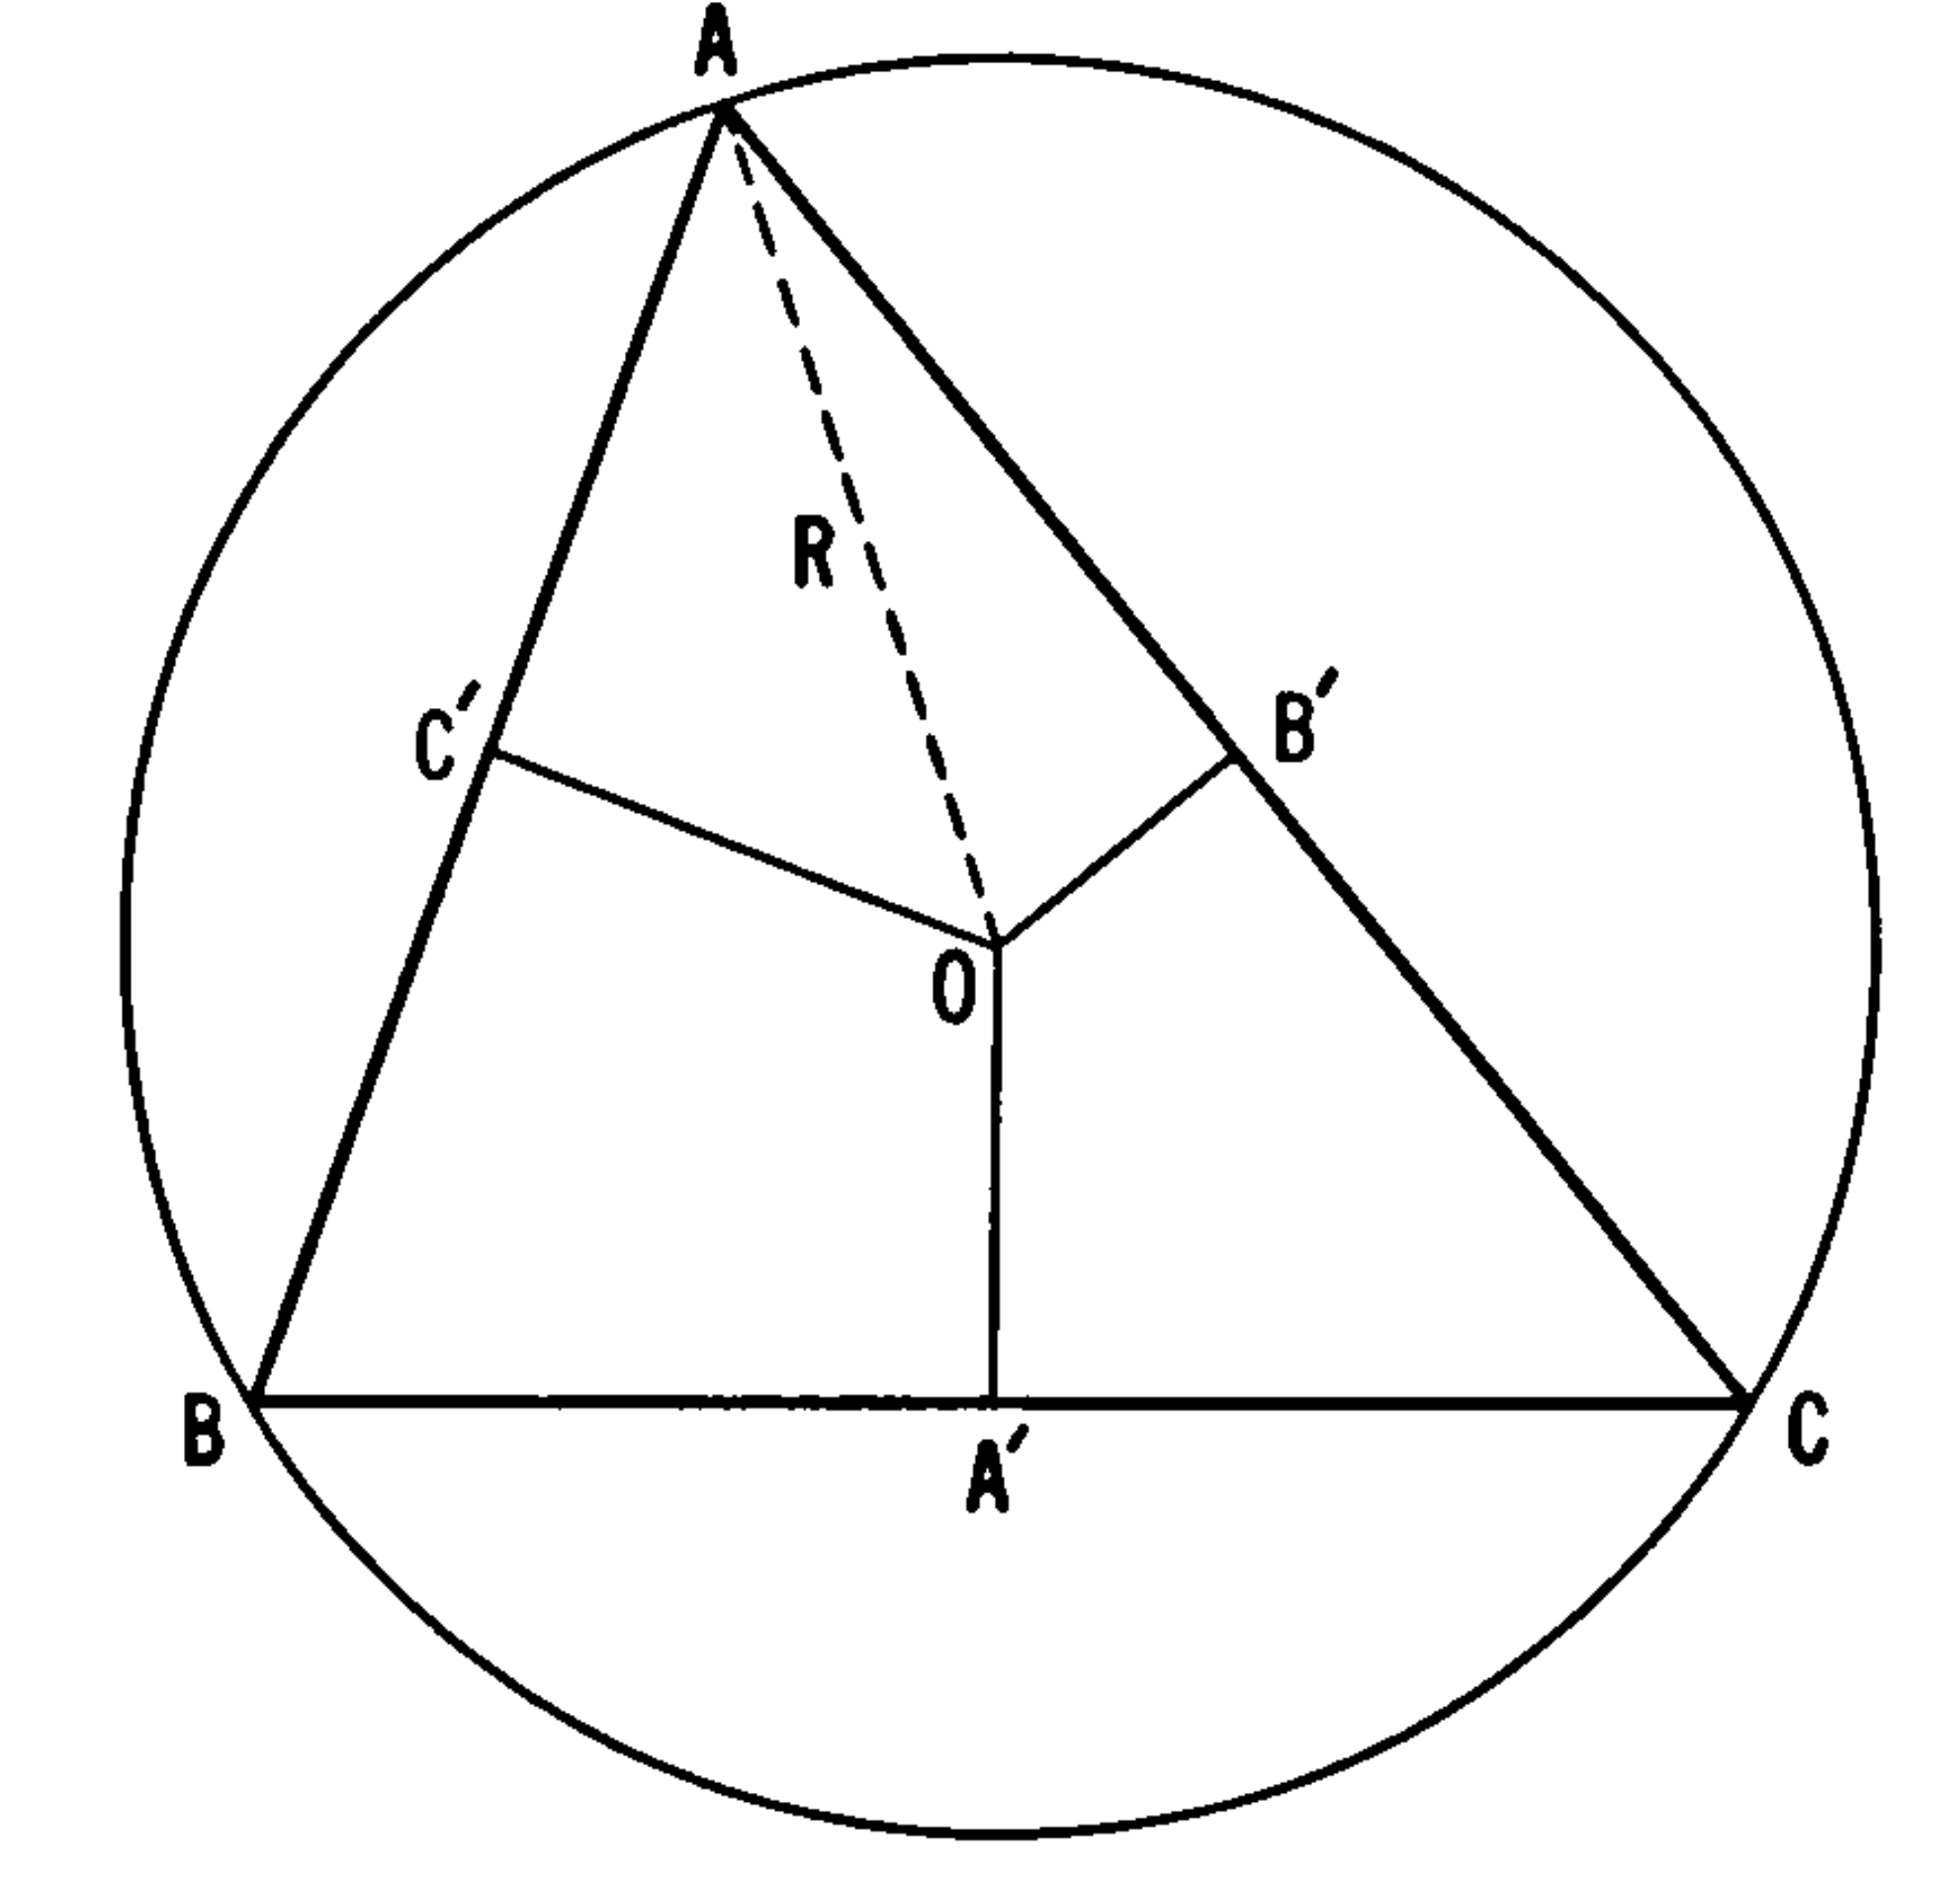
\includegraphics[width=0.4\textwidth]{media/1-3A}
% \end{center}

% \subsubsection{The Centroid}

% \begin{definition}
% 	Cevians that join the vertices of a triangle to the midpoints of the opposite sides are called \vocab{medians}. The medians intersect at the \vocab{centroid}, denoted $G$.
% \end{definition}

% \begin{theorem}
% 	A triangle is dissected by its medians into six smaller triangles of equal area.
% \end{theorem}

% \begin{center}
% 		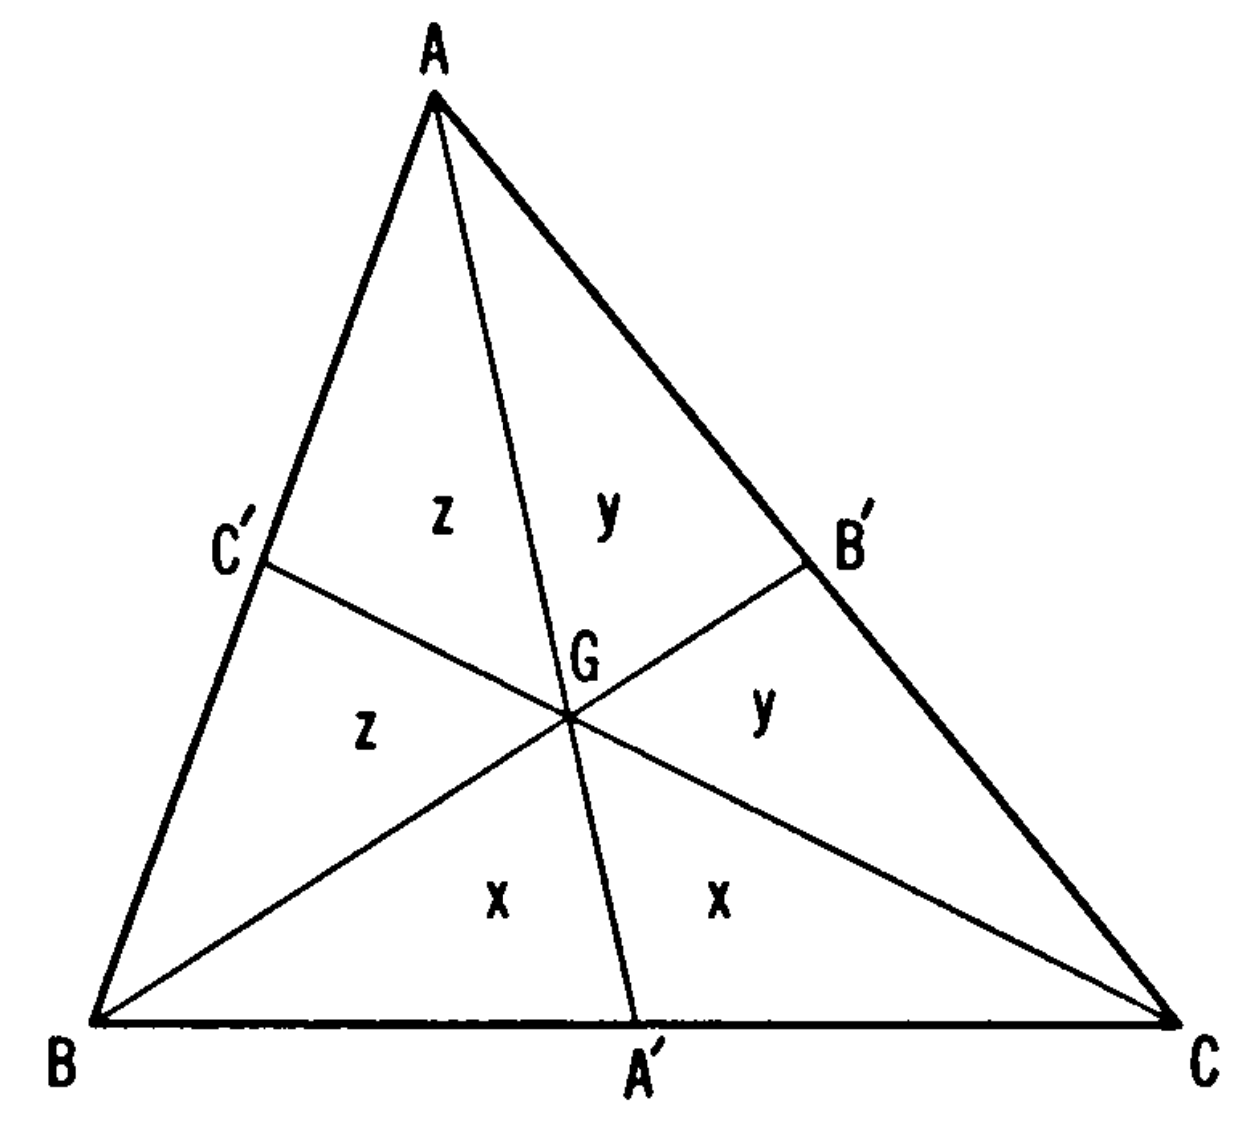
\includegraphics[width=0.4\textwidth]{media/1-3B}
% \end{center}

% \begin{theorem}
% 	The medians of a triangle divide one another in the ratio $2:1$.
% \end{theorem}


% \subsubsection{The Orthocenter}

% \begin{definition}
% 	The cevians $AD$, $BE$, $CF$ perpendicular to $BC$, $CA$, $AB$, respectively are called the \vocab{altitudes} of $\triangle ABS$. Their common point $H$ is the \vocab{orthocenter}.
% \end{definition}

% We also have $\triangle DEF$ named the \vocab{orthic triangle} of $\triangle ABC$. 

% \begin{center}
% 		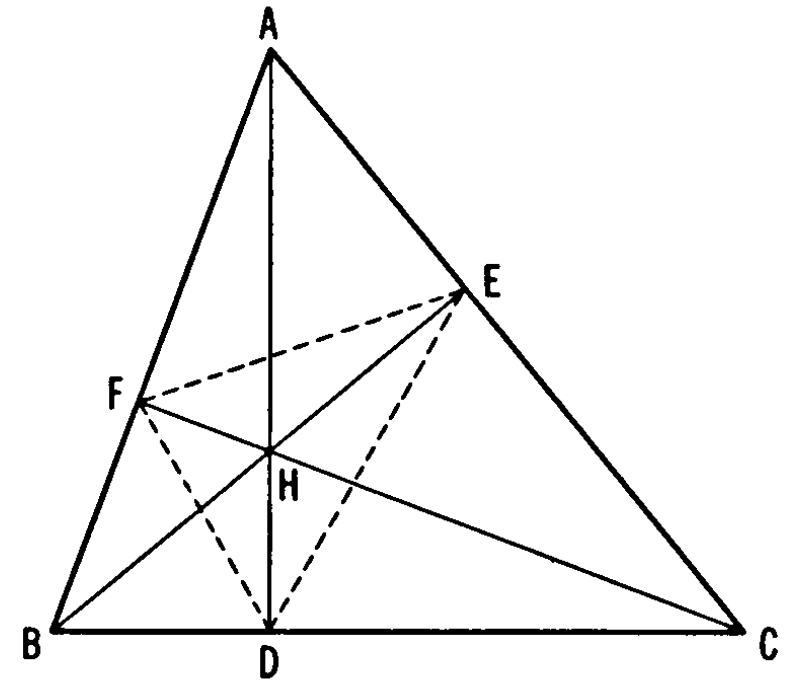
\includegraphics[width=0.4\textwidth]{media/1-3C}
% \end{center}

% \subsubsection{Angle Bisectors and The Incenter}


% \begin{theorem}[Angle Bisector Theorem]
% 	Each angle bisector of a triangle divides the opposite side into segments proportional in length to the adjacent sides.
% \end{theorem}

% For example, in the figure below, we have
% $$
% \frac{BL}{LC}= \frac{c}{b}
% $$

% \begin{center}
  
%       \begin{minipage}[b]{0.45\textwidth}
%     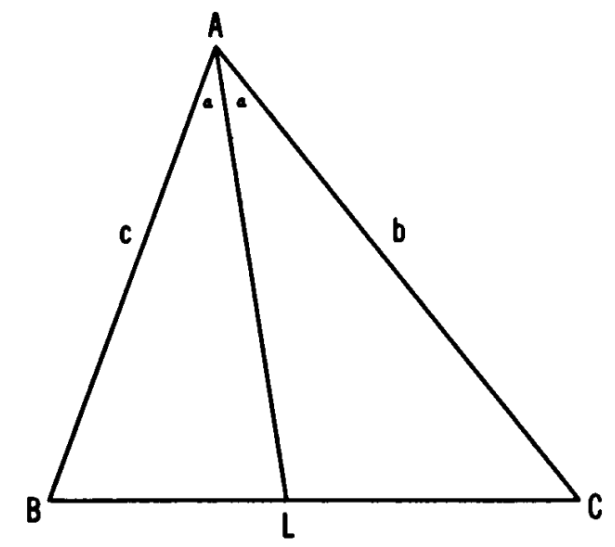
\includegraphics[width=\textwidth]{media/1-3D}
%   \end{minipage}
%   \hfill
%   \begin{minipage}[b]{0.45\textwidth}
%     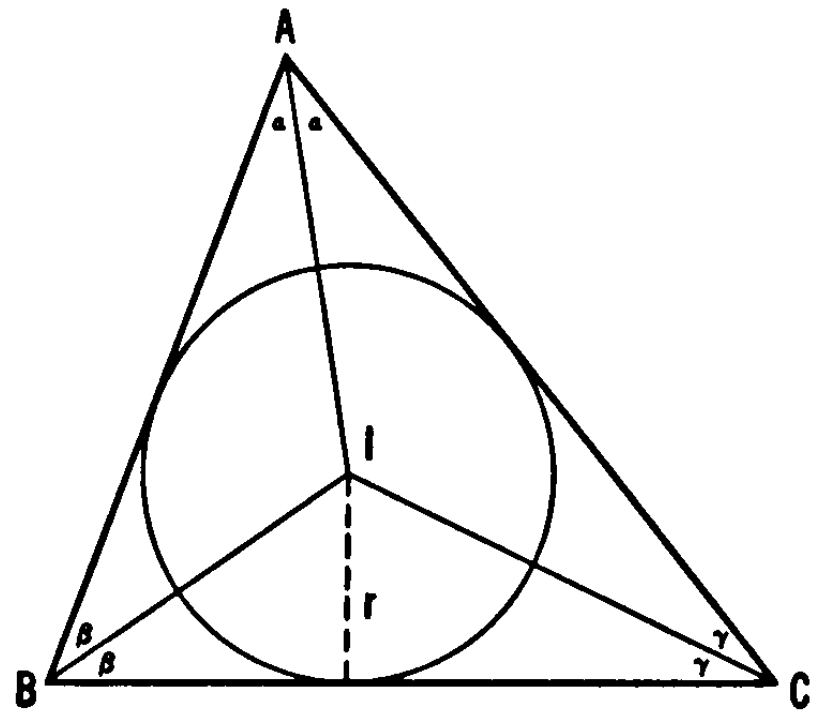
\includegraphics[width=\textwidth]{media/1-3E}
%   \end{minipage}
% \end{center}

% \begin{definition}
% 	The intersection of the angle bisectors $I$ is the center of the inscribed circle, the \vocab{incircle}, whose center is the \vocab{incenter} and radius $r$ is the \vocab{inradius}.
% \end{definition}

% \subsection{Incircles and Excircles}

% \subsubsection{Incircles}

% \begin{definition}
% 	The \vocab{semiperimiter} $s$ is
% 	$$
% s = \frac{a +b + c}{2}.
% $$
% \end{definition}

% \begin{center}
% 		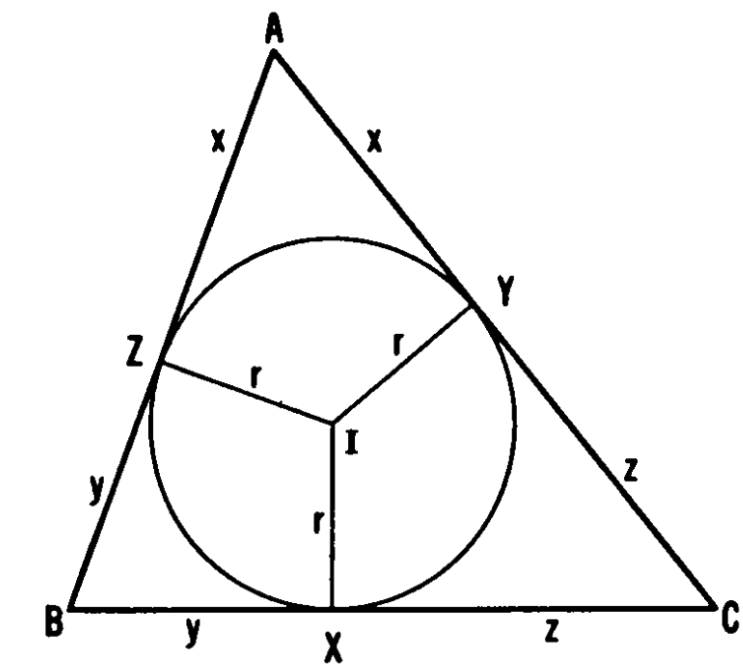
\includegraphics[width=0.4\textwidth]{media/1-4A}
% \end{center}

% \begin{theorem}
% For a triangle $ABC$ whose incircle is tangent to $BC$ at $X$, $AC$ at $Y$ and $AB$ at $Z$,
% 	$$
% 	x = s - a, \quad y = s - b, \quad z =  s - c.
% 	$$
% \end{theorem}

% \begin{theorem}
% 	The area of the triangle $ABC$ is
% 	$
% 	[ABC] = sr.
% 	$
% \end{theorem}

% \begin{theorem}
% 	$
% 	abc = 4srR.
% 	$
% \end{theorem}


% \begin{theorem}
% 	The cevians $AX$, $BY$, $CZ$ are concurrent, with the common point called the \vocab{Gergonne} point of $\triangle ABC$.
% \end{theorem}

% \subsubsection{Excircles}

% Consider the following lemma.
% \begin{lemma}
% 	The external bisectors of any two angles of a triangle are concurrent with the internal bisector of the third angle.
% \end{lemma}

% With this we can define the following points.

% \begin{definition}
% 	Let the \vocab{$a$-excenter} $I_a$ be the intersection of the bisector of $\angle A$ with the external bisectors of $\angle B$ and $\angle C$, and similarly for $I_b$ and $I_c$.
% \end{definition}

% \begin{center}
% 		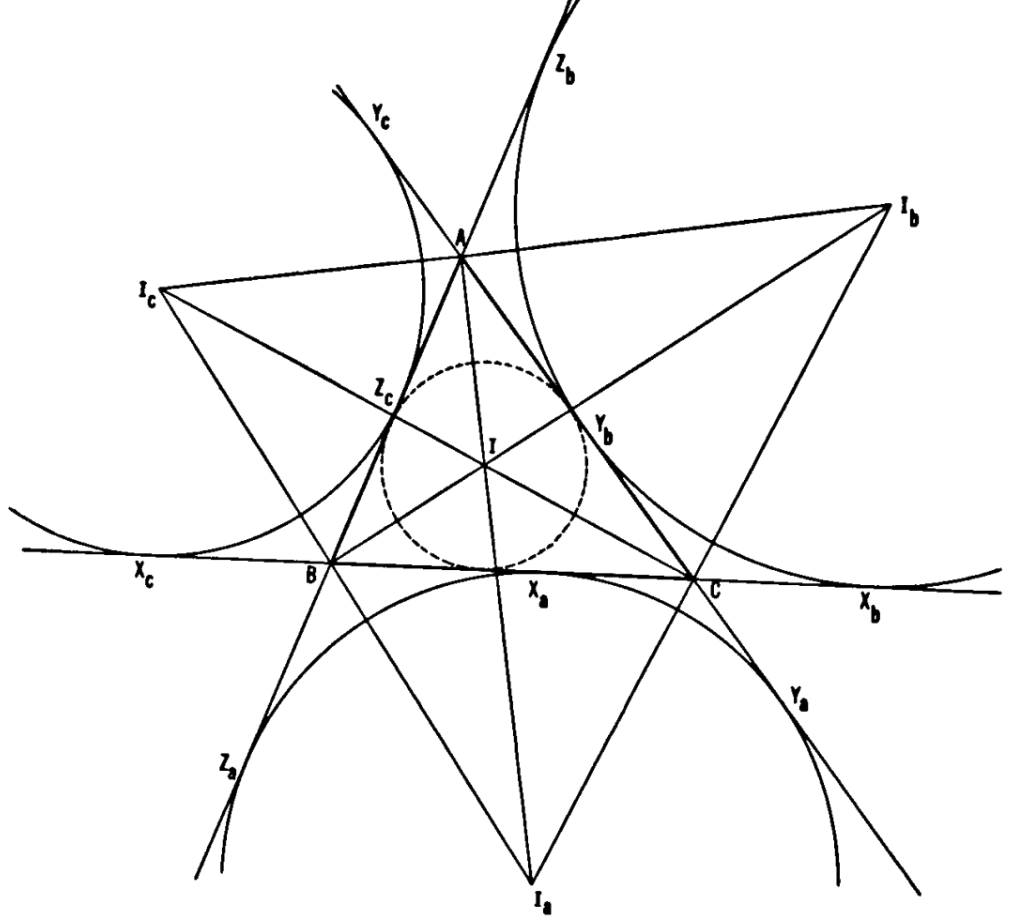
\includegraphics[width=0.8\textwidth]{media/1-4B}
% \end{center}

% \begin{definition}
% 	The circle with center $I_A$ and radius $r_a$, having the extensions of all three sides for tangents is an \vocab{excircle}.
% \end{definition}

% \begin{theorem}
% Using the notation in the diagram above, we have
% 	\begin{align*}
% 		B X_{c}=B Z_{c}=C X_{b}=C Y_{b}&=s-a, \\
% C Y_{a}=C X_{a}=A Y_{c}=A Z_{c}&=s-b, \\
% A Z_{b}=A Y_{b}=B Z_{a}=B X_{a}&=s-c.
% 	\end{align*}
% \end{theorem}

% \begin{lemma}
% 	$\triangle ABC$ is the orthic triangle of $\triangle I_a I_b I_c$.
% \end{lemma}

% \subsection{The Steiner-Lehmus Theorem}

% \begin{theorem}[Steiner-Lehmus]
% 	Any triangle that has two equal angle bisectors (each measured from a vertex to the opposite side) is isosceles.
% \end{theorem}

% \subsection{The Orthic Triangle }

% \begin{center}
% 		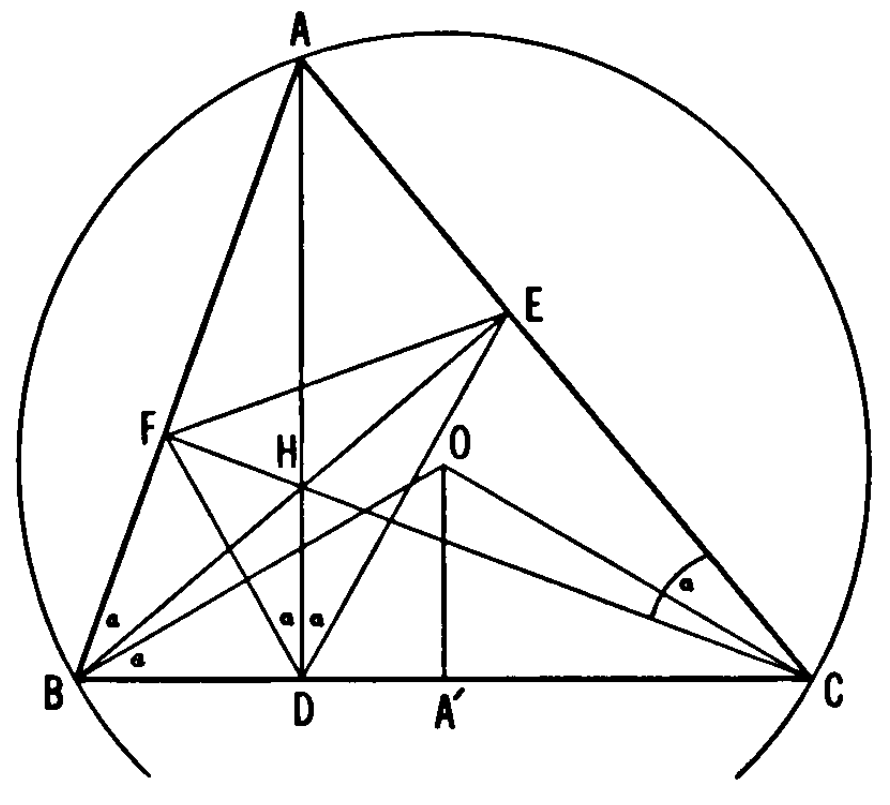
\includegraphics[width=0.5\textwidth]{media/1-6A}
% \end{center}

% \begin{theorem}
% 	The orthocenter of an acute angled triangle is the incenter of its orthic triangle.
% 	The orthocenter of an obtuse angled triangle is an excenter of its othic triangle.
% \end{theorem}

% \begin{lemma}
% 	$\triangle AEF \sim \triangle DBF$, $\triangle DEC \sim \triangle ABC$.
% \end{lemma}

% \subsection{The Medial Triangle and Euler Line}

% \begin{definition}
% 	The triangle formed by joining the midpoints of the sides of a given triangle is the \vocab{medial} triangle.
% \end{definition}

% In the figure below, $\triangle A'B'C'$
%  is the medial triangle of $\triangle ABC$.
 
%  \begin{center}
% 		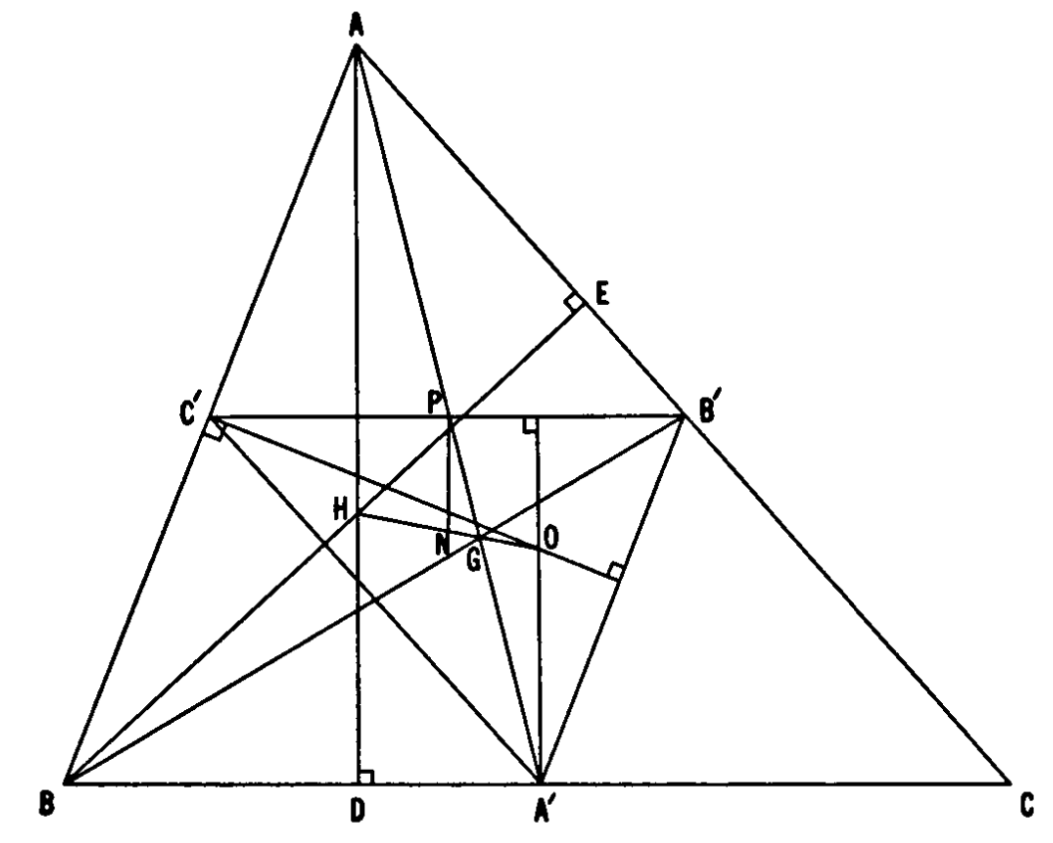
\includegraphics[width=0.5\textwidth]{media/1-7A}
% \end{center}

% \begin{theorem}
% 	$\triangle A'B'C'$ is similar to $\triangle ABC$, in the ratio $1:2$.
% \end{theorem}

% \begin{theorem}[Euler Line]
% 	The orthocenter, centroid and circumcenter of any triangle are collinear. The centroid divides the distance from the orthocenter to the circumcenter in the ratio $2:1$.
% \end{theorem}

% \begin{theorem}
% 	The circumcenter of the medial triangle lies at the midpoint of $HO$ on the Euler line of the parent triangle. Also, since $\triangle A'B'C' \sim \triangle ABC$, the circumradius of the medial triangle is half the cirumradius of the parent triangle.
% \end{theorem}

% \subsection{The Nine Point Circle}

% \begin{theorem}[Nine Point Circle]
% 	The feet of the three altitudes of any triangle, the midpoints of the three sides, and the midpoints of the segments from the three vertices to the orthocenter, all lie on the same circle of radius $\frac{1}{2}R$, the \vocab{nine-point circle}.
% \end{theorem}

% In the figure below, $K$, $L$ and $M$ are the midpoints of the segments from the vertices to the orthocenter.

%  \begin{center}
% 		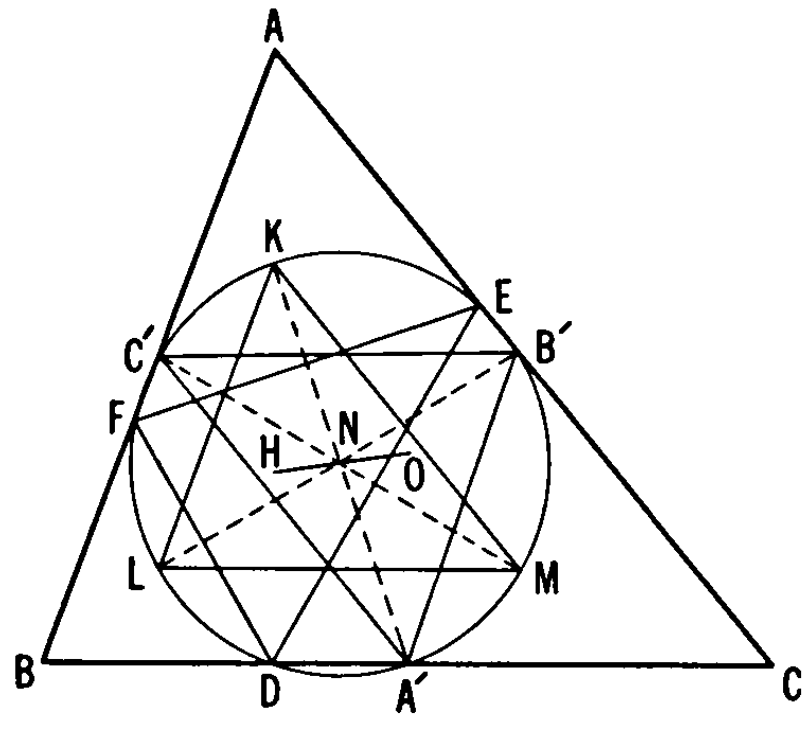
\includegraphics[width=0.5\textwidth]{media/1-8B}
% \end{center}

% \begin{theorem}
% 	The center of the nine-point circle, $N$, lies on the Euler lien, midway between the orthocenter and the circumcenter.
% \end{theorem}

% \begin{theorem}[Feuerbach's Theorem]
% 	The nine-point circle touches the incircle and all four excircles.
% \end{theorem}

% The \vocab{Feuerbach point} is the point of tangency between the incircle and the nine-point circle.

% \begin{lemma}
% 	The quadrilateral $AKA'O$ is a parallelogram.
% \end{lemma}

% \begin{lemma}
% 	The points $K$, $L$ and $M$ bisect the arcs $EF$, $FD$ and $DE$.
% \end{lemma}

% \begin{lemma}
% 	The circumcircle of $\triangle ABC$ is the nine-point circle of $\triangle I_a I_b I_c$.
% \end{lemma}

% \section{Some Properties of Circles}

% \subsection{Power of a Point}

% \begin{theorem}[Intersecting Chords]
% 	If two lines through a point $P$ meet a circle at points $A$, $A'$ (possibly coincident) and $B, B'$ (possible coincident) respectively, then
% 	$$
% 	PA \cdot PA' = PB \cdot PB'
% 	$$
% \end{theorem}

%  \begin{center}
% 		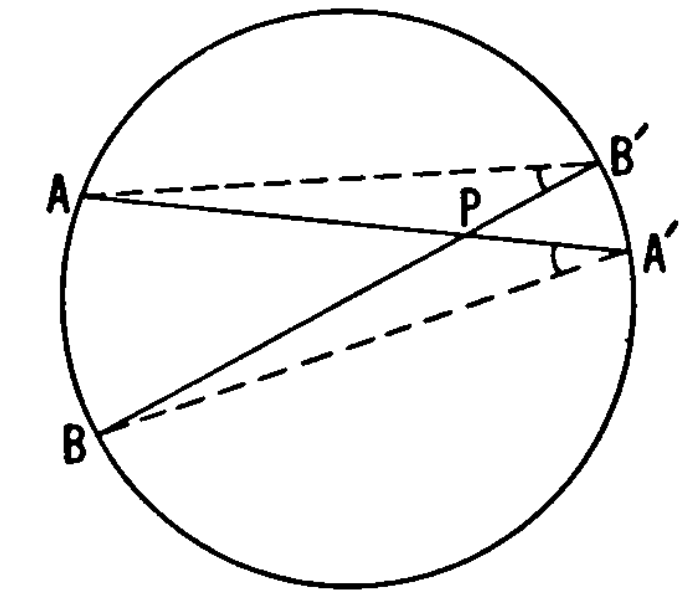
\includegraphics[width=0.4\textwidth]{media/2-1A}
% \end{center}

% \begin{definition}[Power of a Point]
% 	For any circle of radius $R$ and any point $P$ distant $d$ away from the center, we call
% 	$$
% 	d^2 - R^2
% 	$$
% 	the \vocab{power} of $P$ with respect to the circle.
% \end{definition}

% The power of $P$ is clearly positive when $P$ is outside the circle, negative when $P$ is inside, and zero when $P$ lies on the circumference.

% We note that using directed lengths\footnote{Directed lengths is when we assign a `direction' to segments such that $AP = - PA$},
% $$
% d^2 - R^2 = PA \cdot PA'.
% $$

% \subsection{The Radical Axis}

% \begin{theorem}[Existance of the Radical Axis]
% 	The locus of all points whose powers with respect to two nonconcentric circles are equal is a line perpendicular to the line of centers of the two circles.
% \end{theorem}

% We note that if the two circles intersect (or are tangent), then the points of intersections both have zero power with respect to both circles, thus they determine the radical axis.

%  \begin{center}
% 		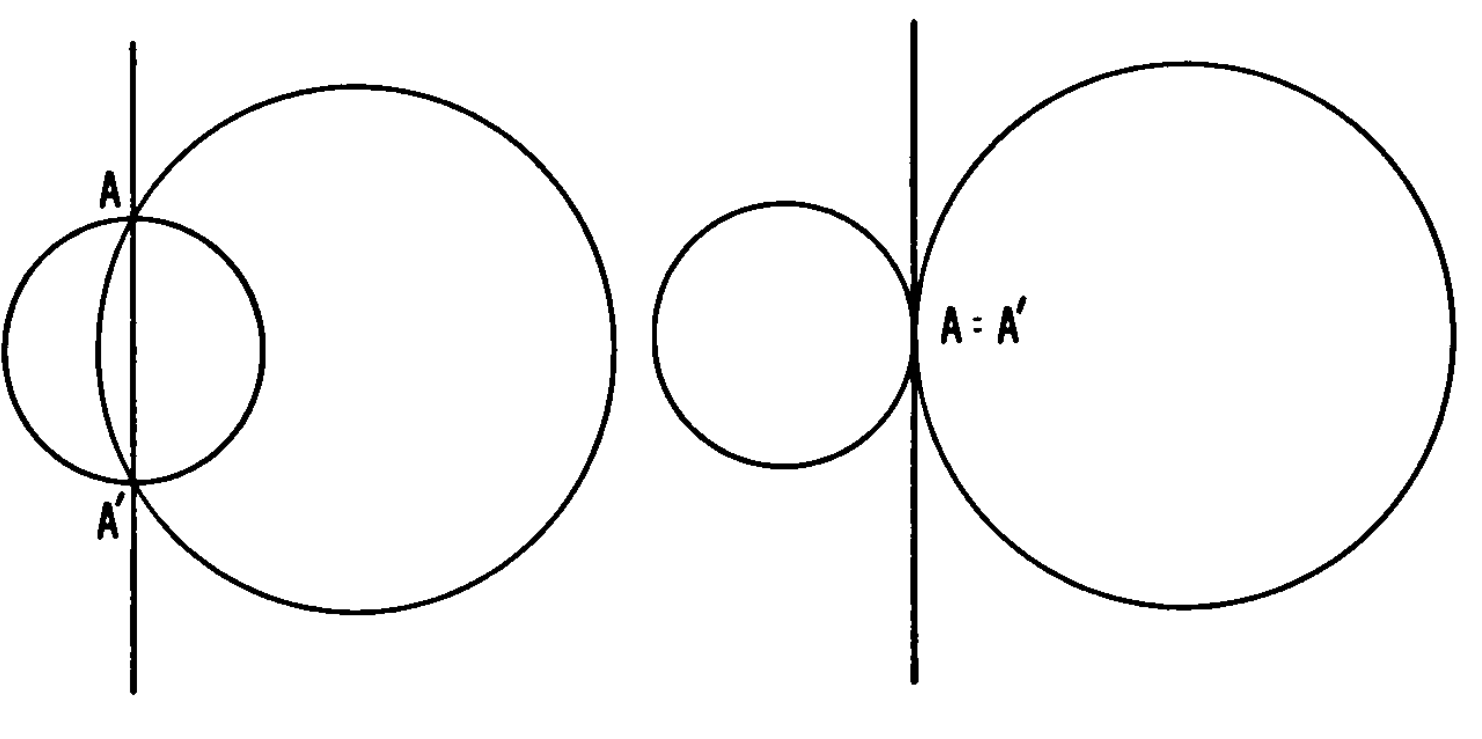
\includegraphics[width=0.6\textwidth]{media/2-2B}
% \end{center}


% \begin{theorem}[Radical Axis Theorem]
% 	If the centers of three circles are not colinear, then there is just one point, the \vocab{radical center} whose powers with respect to all three circles are equal.
% \end{theorem}

% \subsection{Simson Lines}


% \begin{theorem}[Simson Line]
% 	The feet of the perpendiculars from a point to the sides of a triangle are collinear if and only if the point lies on the circumcircle.
% \end{theorem}

%  \begin{center}
% 		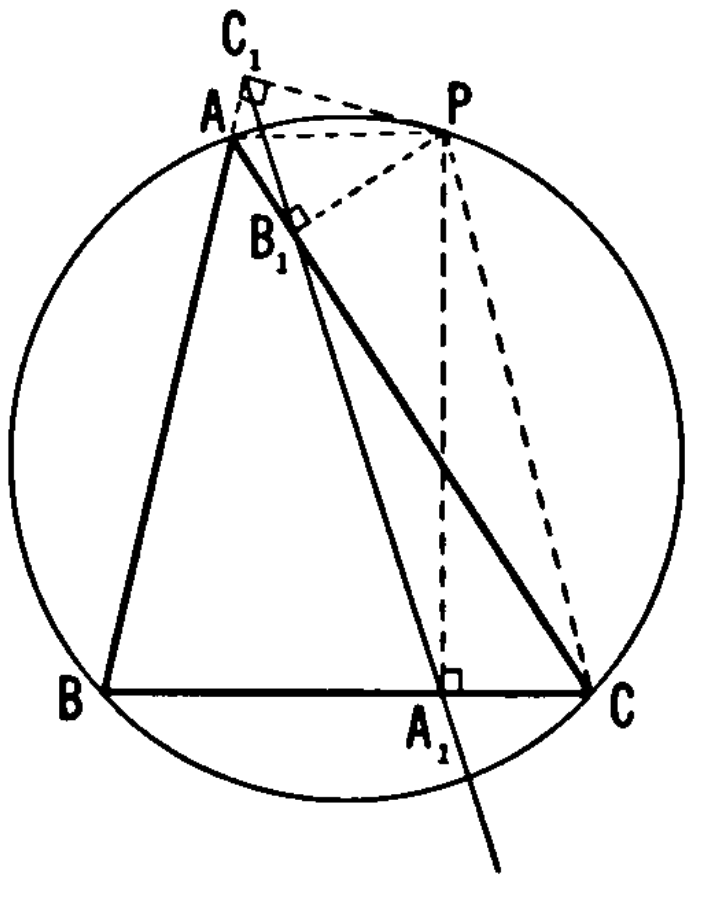
\includegraphics[width=0.3\textwidth]{media/2-5A}
% \end{center}

% \begin{theorem}
% 	The angle between the Simson lines of two points $P$ and $P'$ on the circumcircle is half the angular measure of the arc $P' P$. 
% \end{theorem}

% \begin{theorem}
% 	The Simson line of a point on the circumcircle bisects the segment joining that point to the orthocenter.
% \end{theorem}

% \begin{lemma}
% The Simson lines of diametrically opposite points on the circumcircle are perpendicular to each other and meet on the nine-point circle.
% \end{lemma}



% \subsection{Ptolemy's Theorem}

% \begin{theorem}[Ptolemy]
% 	If a quadrilateral $ABCD$ (in that order) is inscribed in a circle, then
% 	$$
% 	AB \cdot CD + BC \cdot DA = AC \cdot BD.
% 	$$
% \end{theorem}

% The converse of Ptolemy's theorem is true, and we can strengthen its converse using the triangle inequality.

% \begin{theorem}
% 	If $ABC$ is a triangle and $P$ is not on the arc $CA$ of its circumcircle, then
% 	$$
% 	AB \cdot CP + BC \cdot AP > AC \cdot BP.
% 	$$
% \end{theorem}

% \section{Collinearity and Concurrence}

% \subsection{Quadrilaterals and Varignon's Theorem}

% \begin{theorem}[Varignon Parallelogram]
% 	The figure formed when the midpoints of the sides of a quadrilateral are joined in order is a parallelogram, and its area is half that of the quadrilateral.
% \end{theorem}

%  \begin{center}
% 		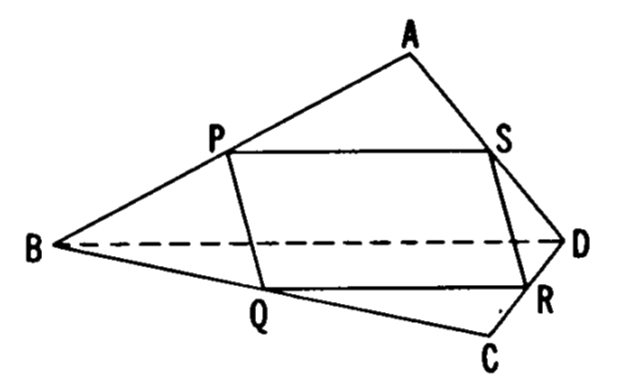
\includegraphics[width=0.4\textwidth]{media/3-1B}
% \end{center}

% \begin{lemma}
% 	The perimeter of the Varignon parallelogram equals the sum of the diagonals of the original quadrilateral.
% \end{lemma}

% \begin{theorem}
% 	The segments joining the midpoints of the pairs of opposite sides of a a quadrilateral and the segment joining the midpoints of the diagonals are concurrent and bisect one another. 
% \end{theorem}

% \begin{theorem}
% 	If one diagonal divides a quadrilateral into two triangles of equal area, it bisects the other diagonal.
% \end{theorem}

%  \begin{center}
% 		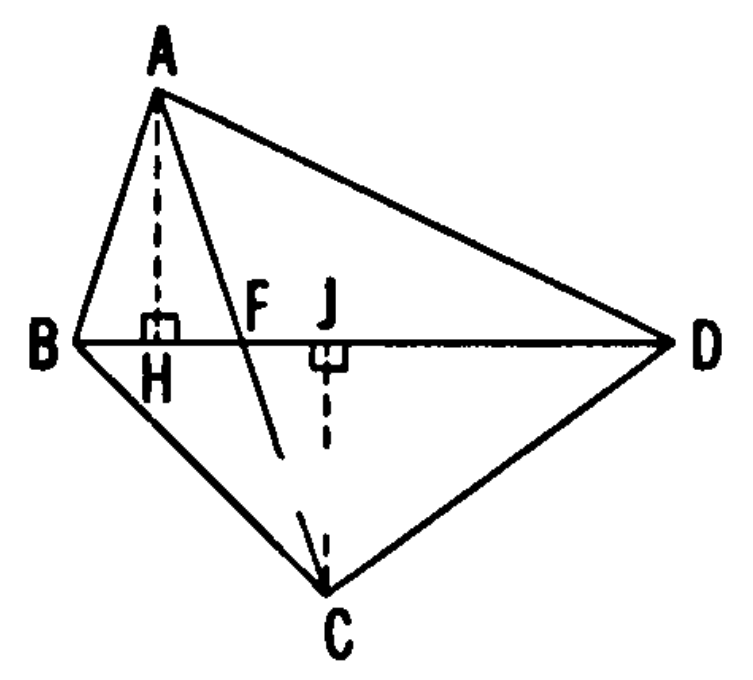
\includegraphics[width=0.3\textwidth]{media/3-1D}
% \end{center}

% Note that the converse of this theorem is also true.

% \begin{theorem}
% 	If a quadrilateral $ABCD$ as its opposite sides $AD$ and $BC$ (extended) meeting at $W$, while $X$ and $Y$ are the midpoints of diagonals $AC$ and $BD$, then
% 	$[WXY] = \frac{1}{4}[ABCD]$
% \end{theorem}

%  \begin{center}
% 		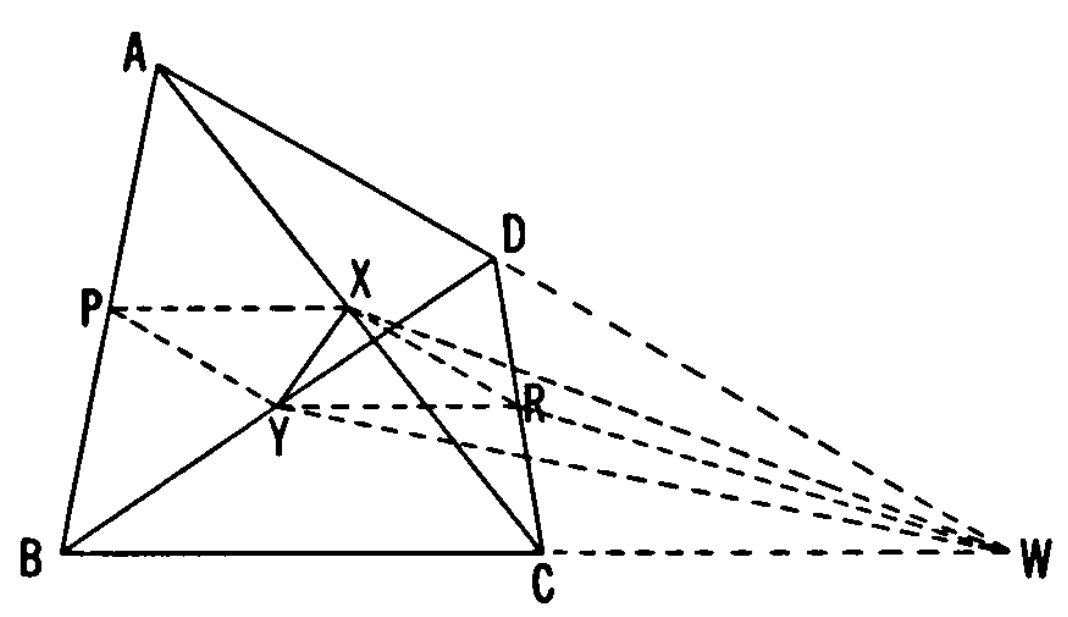
\includegraphics[width=0.55\textwidth]{media/3-1E}
% \end{center}

% \subsection{Cyclic Quadrilaterals and Brahmagupta's Formula}

% \begin{theorem}[Brahmagupta's Formula]
% 	If a cyclic quadrilateral has sides $a$, $b$, $c$, $d$ and semiperimeter $s$, its area is given $K$ by
% 	$$
% 	K = \sqrt{(s - a)(s - b)(s - c)(s - d).}
% 	$$
% \end{theorem}

%  \begin{center}
% 		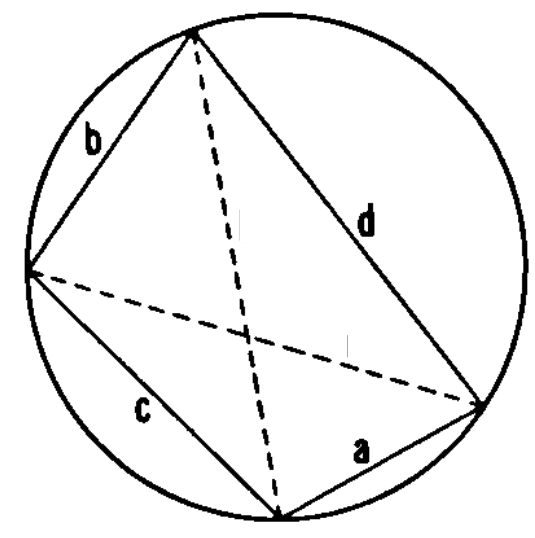
\includegraphics[width=0.3\textwidth]{media/3-2A}
% \end{center}

% \begin{corollary}[Heron's formula]
% 	The area of a triangle $ABC$ with sidelengths $a$, $b$, $c$ and semiperimeter $s$ is
% 	$$
% 	[ABC] = \sqrt{s(s - a)(s - b)(s - c)}
% 	$$
% \end{corollary}

% \begin{theorem}
% 	If a cyclic quadrilateral has perpendicular diagonals crossing at $P$, the line through $P$ perpendicular to any side bisects the opposite side.
% \end{theorem}

%  \begin{center}
% 		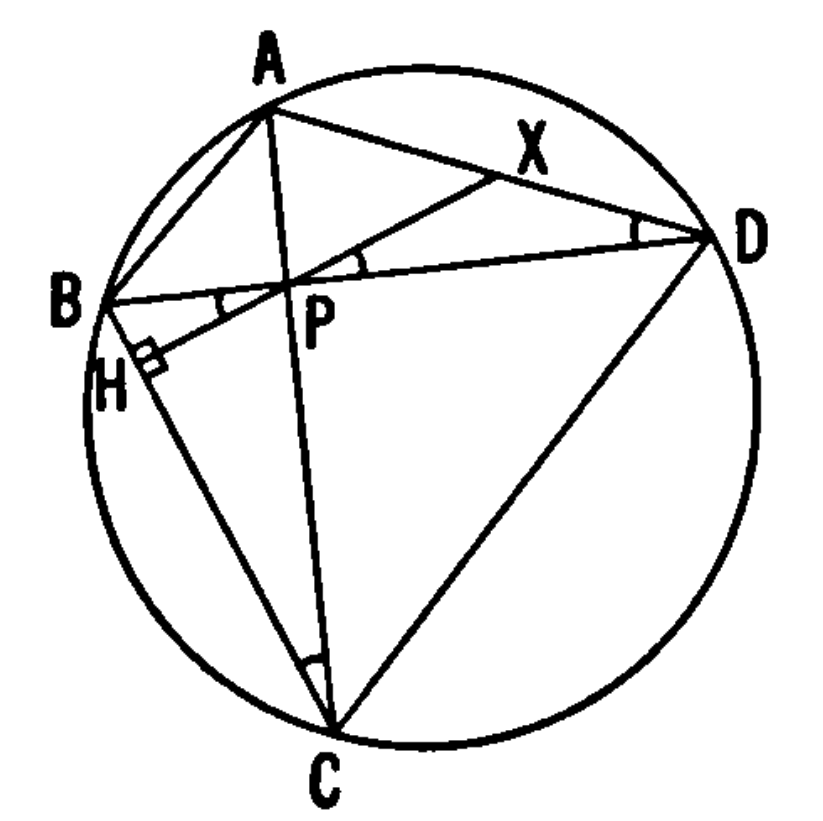
\includegraphics[width=0.28\textwidth]{media/3-2C}
% \end{center}

% \subsection{Napoleon Triangles}

% \begin{theorem}
% Let triangles be erected externally on the sides of an arbitrary triangle so that the sum of the ``remote" angles of these three triangles is $180^{\circ}$. Then the circumcircles of the three triangles have a common point.
% \end{theorem}

%  \begin{center}
% 		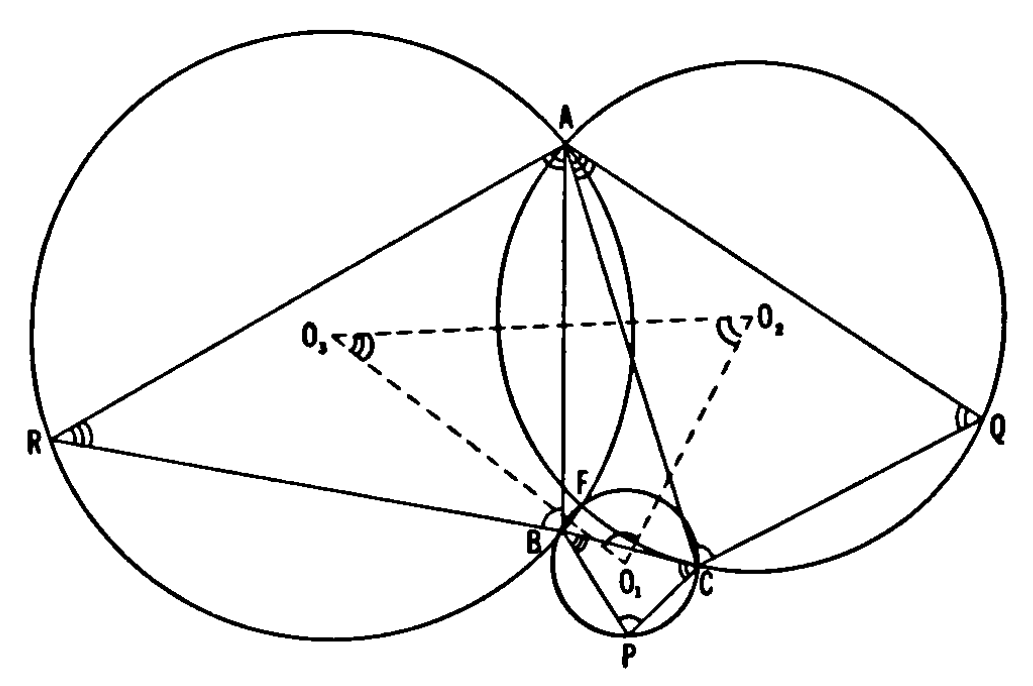
\includegraphics[width=0.6\textwidth]{media/3-3A}
% \end{center}

% This has a particularly important corrolary. If the vertices of $A, B, C$ of $\triangle ABC$ lie on sides $QR, PR$ and $PQ$ respectively of $\triangle PQR$, then the circles $CBP$, $ACQ$ and $BAR$ have a common point.
% Phrased differently, 

% \begin{corollary}[Miquel's Theorem]
% 	Let $ABC$ be a triangle and let $X$, $Y$, $Z$ be points on sides $AB$, $BC$ and $AC$ respectively. Then the circles $AXZ$, $XYB$ and $ZYC$ pass through a common point, called the \vocab{Miquel point}. 
% \end{corollary}

% \begin{theorem}[Miquel's Quadrilateral Theorem]
% 	IF four lines meet one another at six points $A, B, C, A_1, B_1, C_1$, so that the sets of collinear points are $A_1 BC$, $AB_1C$, $ABC_1$, $A_1 B_1 C_1$, then the four circles $AB_1 C_1$, $A_1 B C_1$, $A_1 B_1 C$, $ABC$ have a common point.
% \end{theorem}

% We also have this theorem, and it's generalization

% \begin{theorem}[Napoleon's Theorem]
% 	If equilaterals are erected externally on the sides of any triangles, their centers form an equilateral triangle.
% \end{theorem}

%  \begin{center}
% 		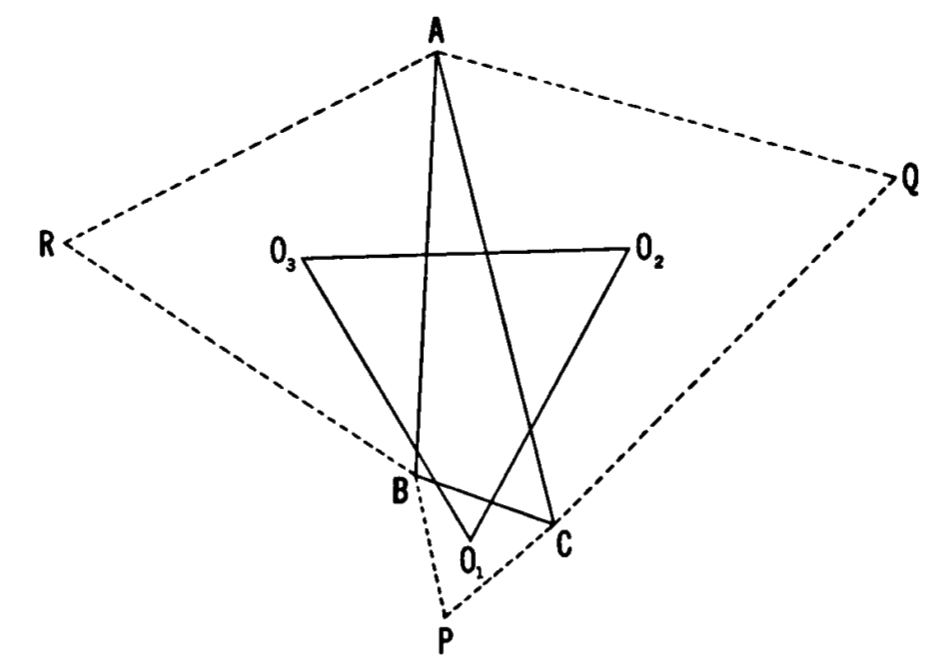
\includegraphics[width=0.6\textwidth]{media/3-3B}
% \end{center}

% \begin{theorem}[Generalized Napoleon's Theorem]
% 	If similar triangles are erected externally on the sides of any triangle, their circumcenters form a triangle similar to the three triangles.
% \end{theorem}

% \subsection{Menelaus's Theorem}

% We can use a similar theorem to Ceva's theorem in order to prove colinearity.

% Using directed segments, we have the following.

% \begin{theorem}[Menelaus's Theorem]
% 	Points $X, Y, Z$ on the sides $BC$, $CA$, $AB$ (extended) of $\triangle ABC$ are collinear if and only if
% 	$$
% 	\frac{BX}{XC} \cdot \frac{CY}{YA} \cdot \frac{AZ}{ZB} = -1.
% 	$$ 
% \end{theorem}

%  \begin{center}
% 		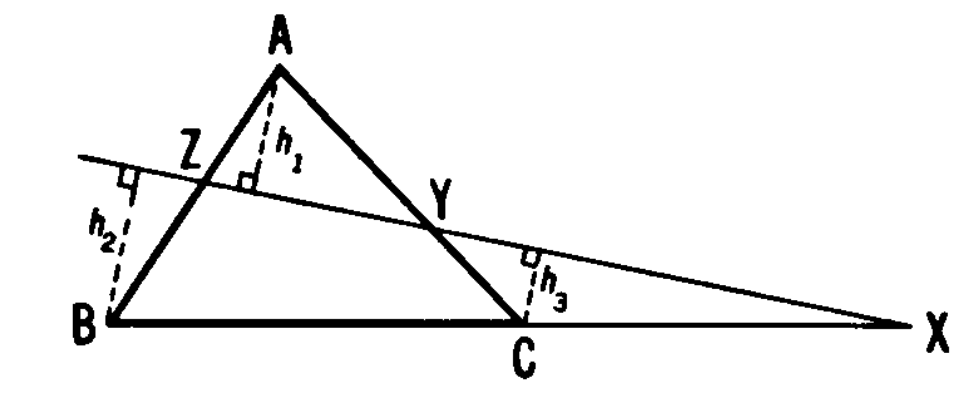
\includegraphics[width=0.5\textwidth]{media/3-4B}
% \end{center}


% \subsection{Pappus's Theorem}

% \begin{theorem}[Pappus's Theorem]
% 	If $A$, $C$, $E$ are three points on one line, $B$, $D$, $F$ on another, and if the three lines $AB$, $CD$, $EF$ meet $DE$, $FA$, $BC$ respectively, then the three points of intersection $L$, $M$, $N$ are collinear.
% \end{theorem}

%  \begin{center}
% 		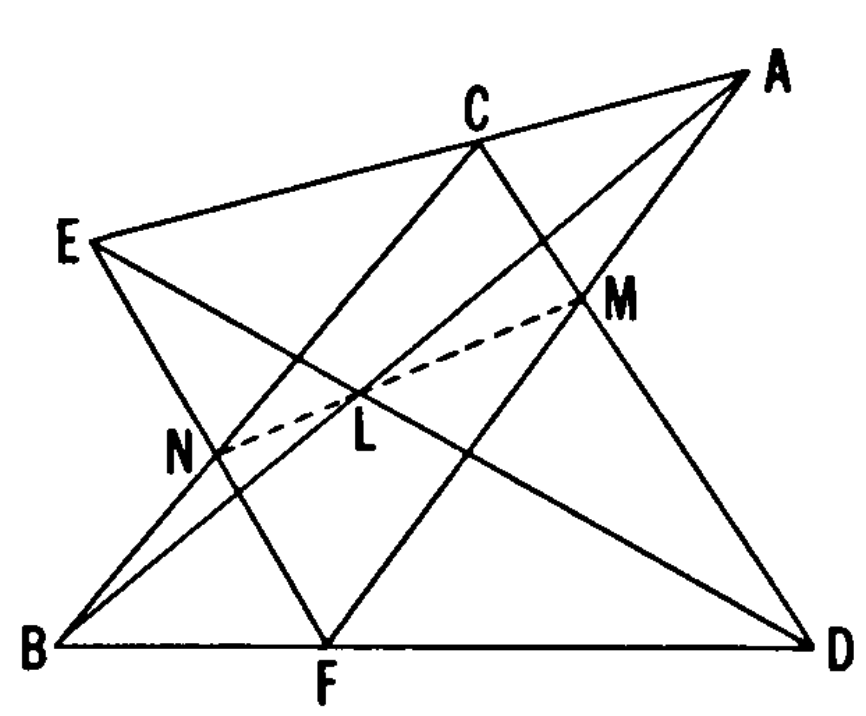
\includegraphics[width=0.5\textwidth]{media/3-5A}
% \end{center}

% \subsection{Perspective Triangles and Desargues's Theorem}

% \begin{theorem}[Desargues's Theorem]
% 	If two triangles are in perspective from a point, and if their pairs of corresponding sides meet, then the three points of intersection are collinear.
% \end{theorem}

%  \begin{center}
% 		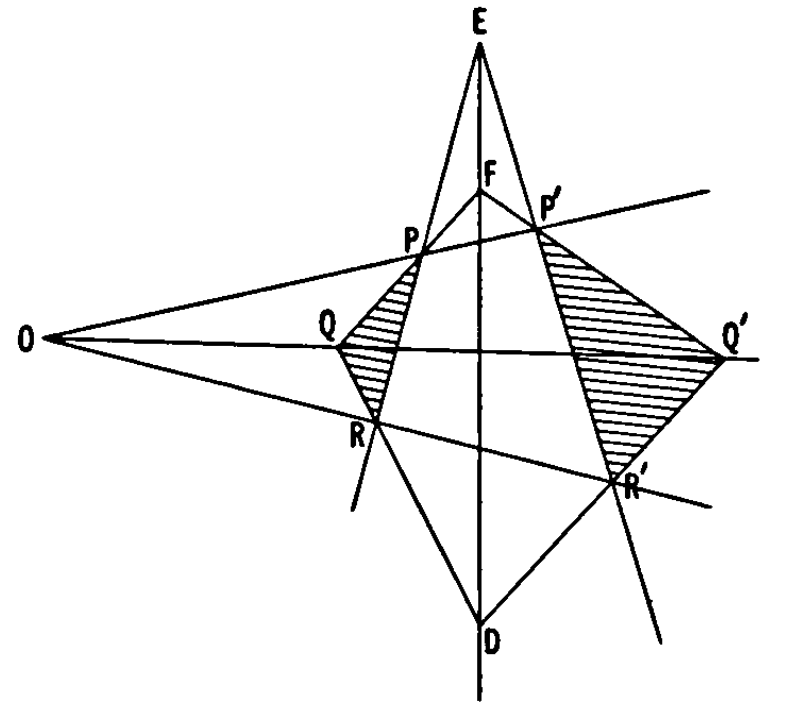
\includegraphics[width=0.4\textwidth]{media/3-6A}
% \end{center}

% We also have the converse.

% \begin{theorem}[Converse to Desargues's Theorem]
% 	If two triangles are in perspective from a line, and if two pairs of corresponding vertices are joined by intersecting lines, the triangles are in perspective from a point of intersection of these lines.
% \end{theorem}

% \subsection{Pascal's Theorem}


% \begin{theorem}[Pascal's Theorem]
% If all six vertices of a hexagon lie on a circle and the three pairs of opposite sides intersect, then the three points of intersection are collinear.
% \end{theorem}

%  \begin{center}
% 		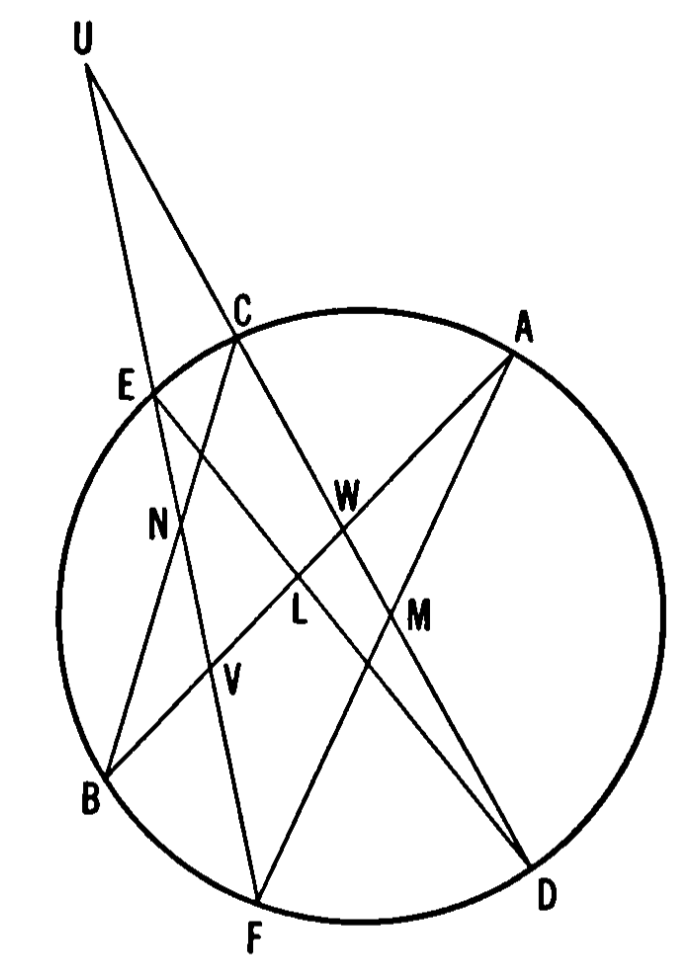
\includegraphics[width=0.35\textwidth]{media/3-8A}
% \end{center}

% In fact a stronger theorem is true, which is that if the vertices of the hexagon lie on a conic then the three points of intersection are collinear. The converse of this stronger theorem is true (that colinear intersection of opposite sides of a hexagon implies the vertices lie on a conic).



%\begin{problem}
% Two circles are in contact internally at a point $T$. Let the chord $A B$ of
%the larger circle be tangent to the smaller circle at a point $P .$ Then the line $T P$ bisects $\angle A T B$.
%\end{problem}
%
%\textbf{Solution.}
%
%\begin{itemize}
%	\item Let $C$ be the second point of intersection between $BT$ and the smaller circle.
%	\item Take the homothety from $TCP$ to $TBP'$.
%	\item As $T$ and the centers of the two circles are colinear, this homothety takes the smaller circle to the larger circle, and thus $P'$ lies on the larger circle.
%	\item Due to our homothety, we have $\angle TPC = \angle TP'B = \angle TAB$.
%	\item By angle in the alternate segment, $\angle BPC = \angle PTC$, and $\angle APT = \angle PCT$
%	\item Thus $\angle ATP = \angle PTC$, so $TP$ bisects $\angle ATC$.
%\end{itemize}
	



\end{document}
